\chapter{Funktionsweise \label{chap_funktionsweise}}
\ac{ITS} besteht aus verschiedenen Komponenten. Diese Komponenten können mobil oder stationär sein. Die Grafik \ref{fig:funktionsweise_komponentenueberblick} gibt einen Überblick über die in \ac{ITS} verwendeten Komponenten. Jede dieser Komponenten stellt eine \ac{ITS-S} dar. \ac{ITS-S} bezeichnet allgemein einen Teilnehmer des \ac{ITS} Systems. Dieser Abschnitt bezieht sich hauptsächlich auf die \ac{ETSI} Standards \cite{en302665} und \cite{etsi302636-3}. Standard \cite{en302665} definiert Funktionalitäten, Standard  \cite{etsi302636-3} definiert die Realisierung dieser Funktionalitäten. Im Folgenden werden die Komponenten beschrieben und anhand von beiden Standards erklärt.


\begin{figure}
	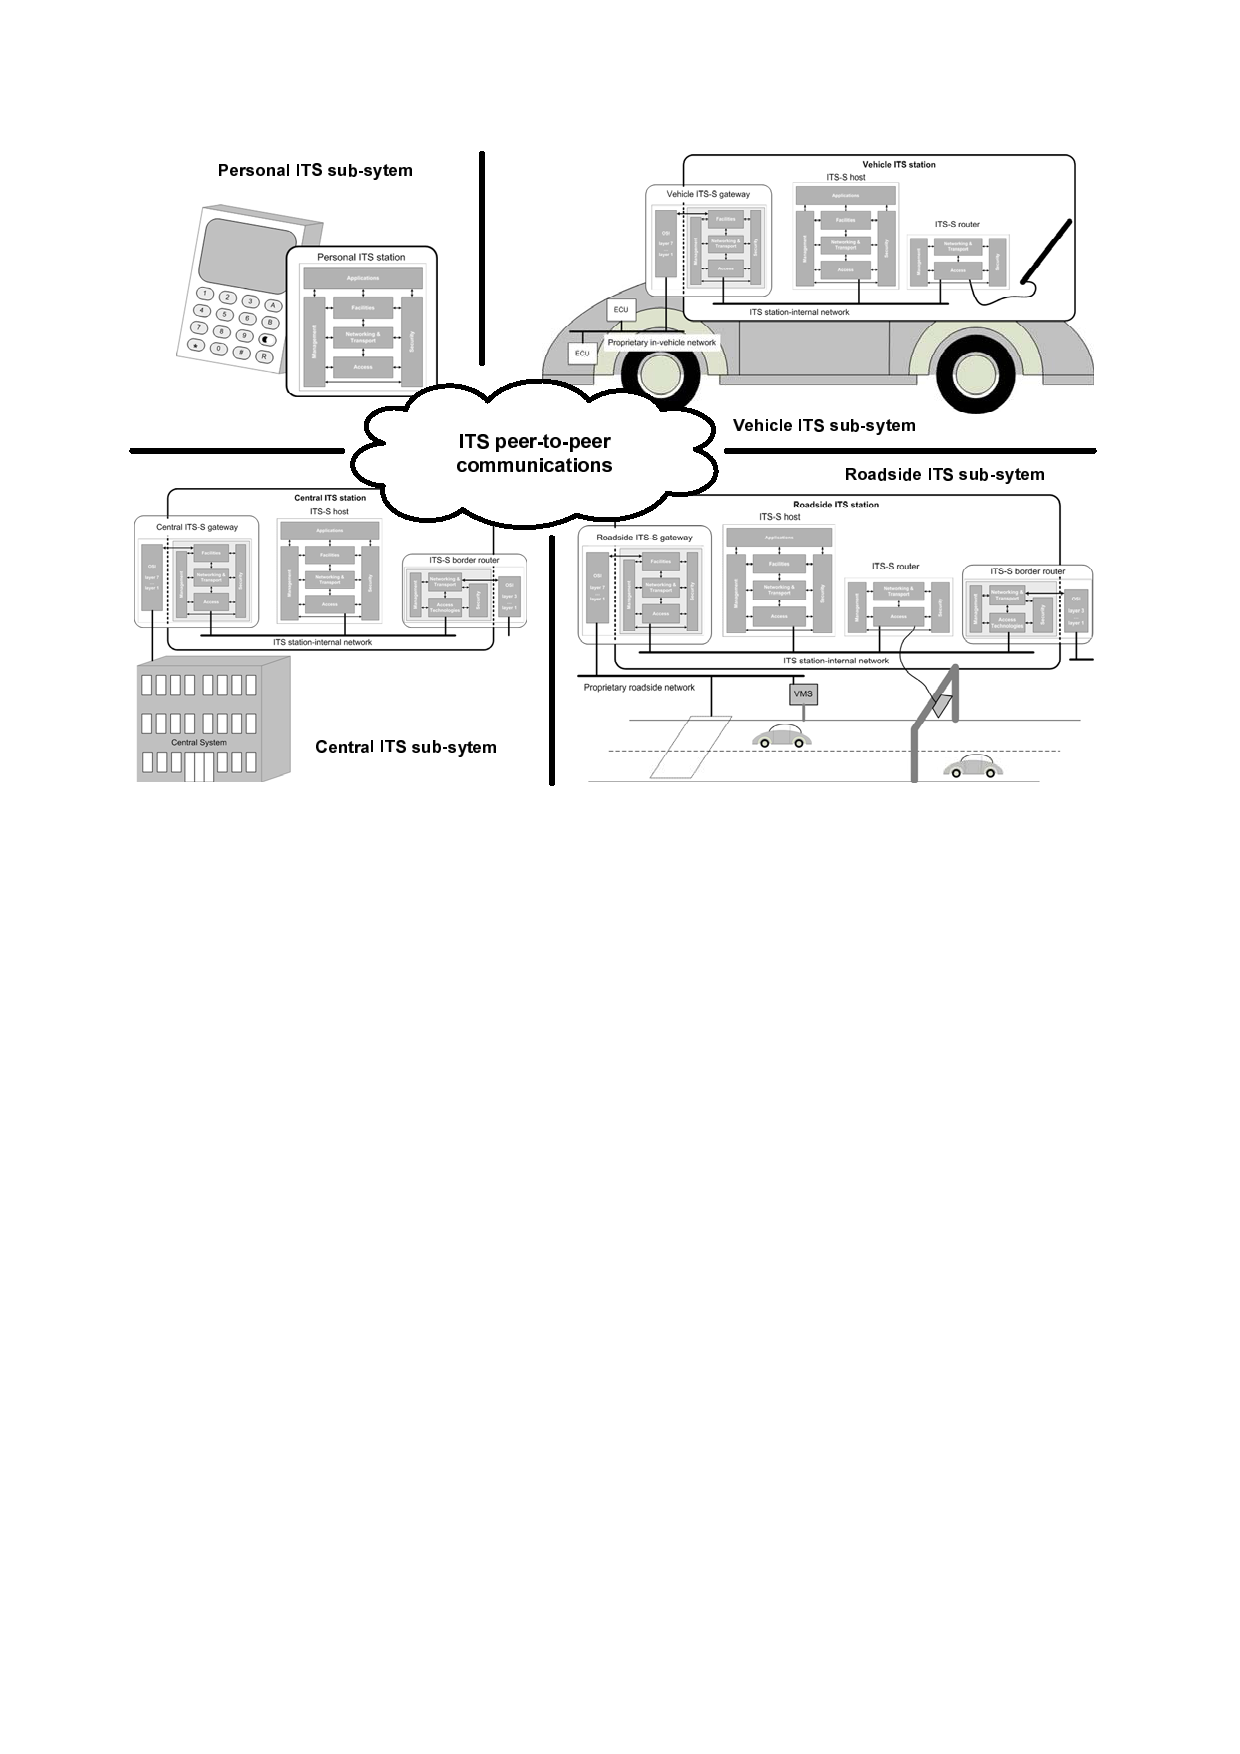
\includegraphics[width=0.99\textwidth]{content/images/01_funktionsweise/ueberblick-ITS-subsystems.pdf}
	\caption{Überblick über die Komponenten \cite{en302665}}
	\label{fig:funktionsweise_komponentenueberblick}
\end{figure}


\section{Funktionale Komponenten von ITS \label{funktionsweise_funktionaleKomponenten}}
Die funktionalen Komponenten sind in sich geschlossene Einheiten, die in den \ac{ITS} Subsystems vorhanden sind. Sie werden anhand ihrer Aufgaben und Funktionen getrennt. Dabei muss nicht zwangsläufig eine physikalische Trennung stattfinden, prinzipiell können auch alle funktionalen Komponenten in ein Gerät implementiert werden. Eine genaue Vorschrift der Implementierung sieht der Standard nicht vor, diese Entscheidung liegt bei den \ac{OEM}. 

Neben den Subsystems selber wird auch beschrieben, welche von ihnen als Mindestanforderung in einer \ac{ITS-S} vorhanden sein müssen.

Auf die einzelnen Layer der Komponenten wird im \autoref{chap_archtitektur} eingegangen.   

\subsection{ITS-S Host \label{funktionsweise_ITSHost}}
Der \ac{ITS-S} Host beinhaltet mindestens die \ac{ITS-S} Anwendungen und die Funktionalität der ITS  Station Reference Architektur, die für die  \ac{ITS-S} Anwendungen gebraucht wird. Konkret sind das der \ac{ITS} Network Layer und der Application Layer. 

Die Funktionalitäten des \ac{ITS-S} Host werden im Standard \cite{etsi302636-3} der \ac{AU} zugesprochen. Sämtliche andere Funktionalitäten sind auf die \ac{CCU} ausgelagert. Diese Aufteilung hängt aber von der zu implementierenden Komponente ab, ein Skalieren muss möglich sein.

\subsection{Roadside ITS-S Gateway \label{funktionsweise_RoadsideITSGateway}}
Die Funktionsweise des Roadside \ac{ITS-S} Gateway ergibt sich aus der Grafik \ref{fig:funktionsweise_itsGateway}. Die Aufgabe ist die Gleiche, wie die der meisten Gateways. Es verbindet unterschiedliche Protokollstacks miteinander. In diesem Fall werden das \ac{ITS} interne Netzwerk und ein proprietäres Netzwerk miteinander verbunden. Das proprietäre Netzwerk kann beispielsweise ein IP basierendes Netzwerk sein.

\begin{figure}[h]
	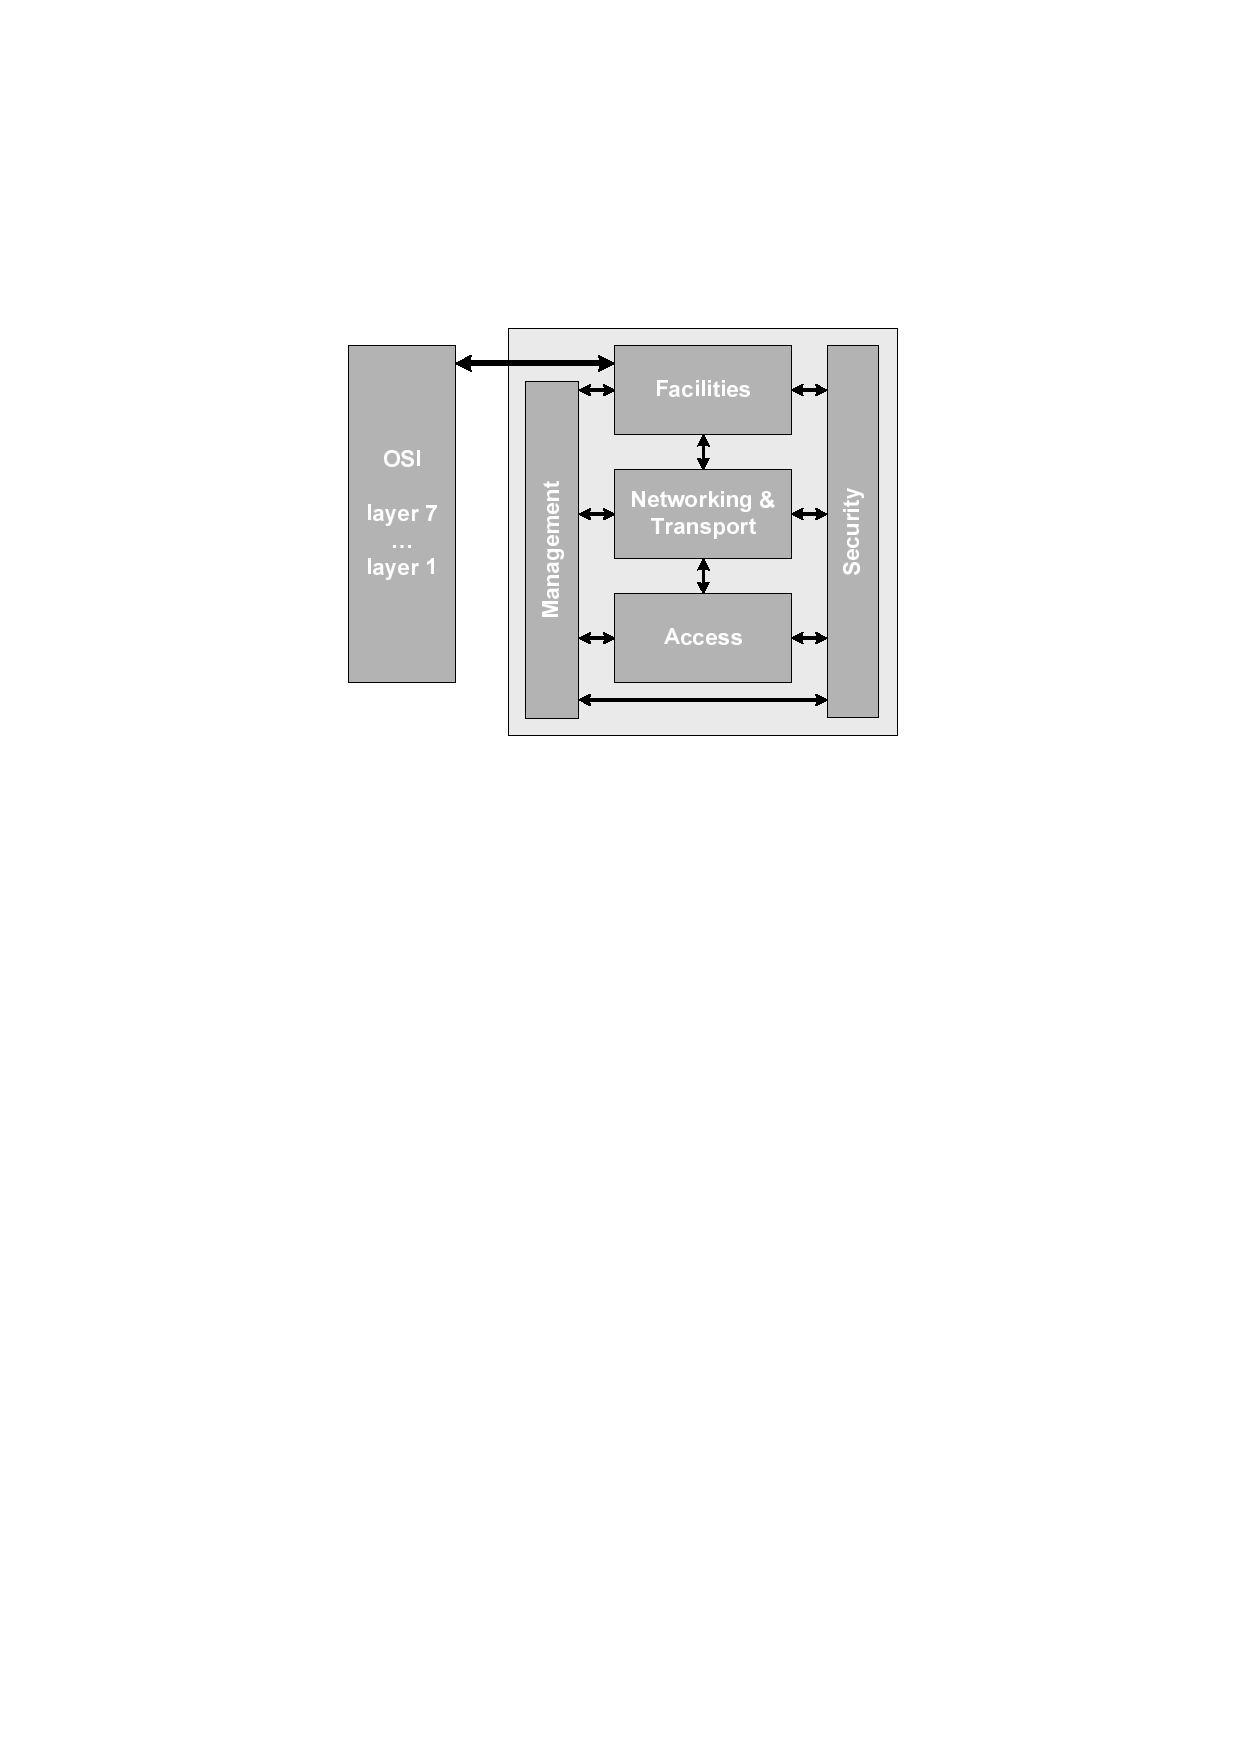
\includegraphics[width=0.75\textwidth]{content/images/01_funktionsweise/layer_gateway.pdf}
	\caption{Überblick über die Layer eines ITS Gateways \cite{en302665}}
	\label{fig:funktionsweise_itsGateway}
\end{figure}


\subsection{ITS-S Router \label{funktionsweise_router}}
Ein \ac{ITS} Router bietet alle Funktionen der \ac{ISO} Referenzarchitektur, ausgenommen die beiden oberen Layer Application und Facilities. Er verbindet zwei unterschiedliche \ac{ITS} Protokoll Stacks auf Layer 3. Einer dieser Protokoll Stacks ist normalerweise mit dem internen \ac{ITS} Netzwerk verbunden. Router werden genutzt um eine Verbindung zu anderen \ac{ITS} Komponenten aufzubauen. Die Darstellung der Layer eines Routers befindet sich in  \autoref{fig:funktionsweise_layerHost}.

\begin{figure}
	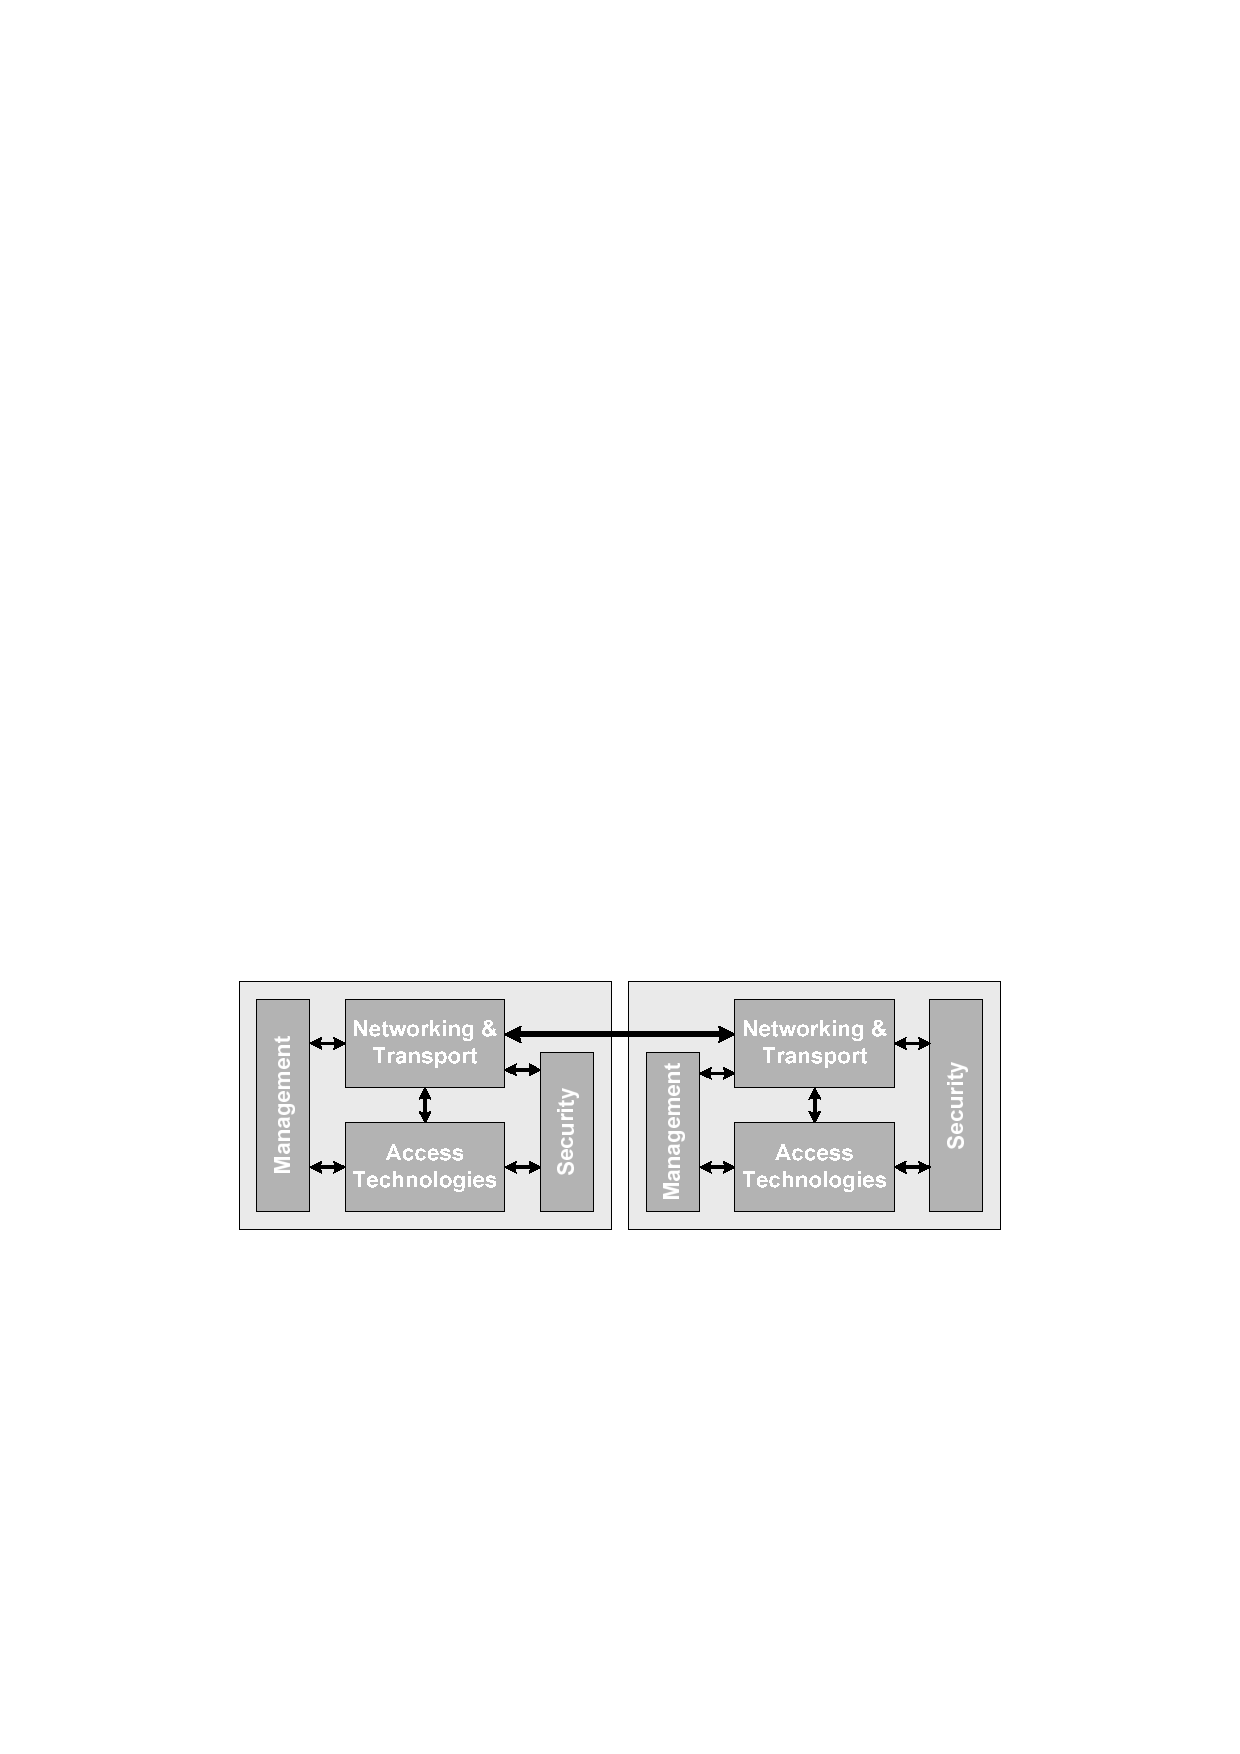
\includegraphics[width=0.99\textwidth]{content/images/01_funktionsweise/layer_router.pdf}
	\caption{Überblick über die Layer eines ITS Routers \cite{en302665}}
	\label{fig:funktionsweise_layerHost}
\end{figure}



\subsection{ITS-S Border Router \label{funktionsweise_ITSBorderRouter}}
Ein Border Router hat die gleichen Funktionalitäten wie ein Router (\autoref{funktionsweise_router}). Der Unterschied ist, dass ein Border Router zwischen einem \ac{ITS} Netz und einem Netz ohne die Cross Layer vermitteln kann. Ein Beispiel für ein solches Netz ist das Internet. Ein Border Router leitet die Datenpakete weiter, verhindert aber einen Einblick in den Aufbau des \ac{ITS} Netzes. 

  
\begin{figure}
	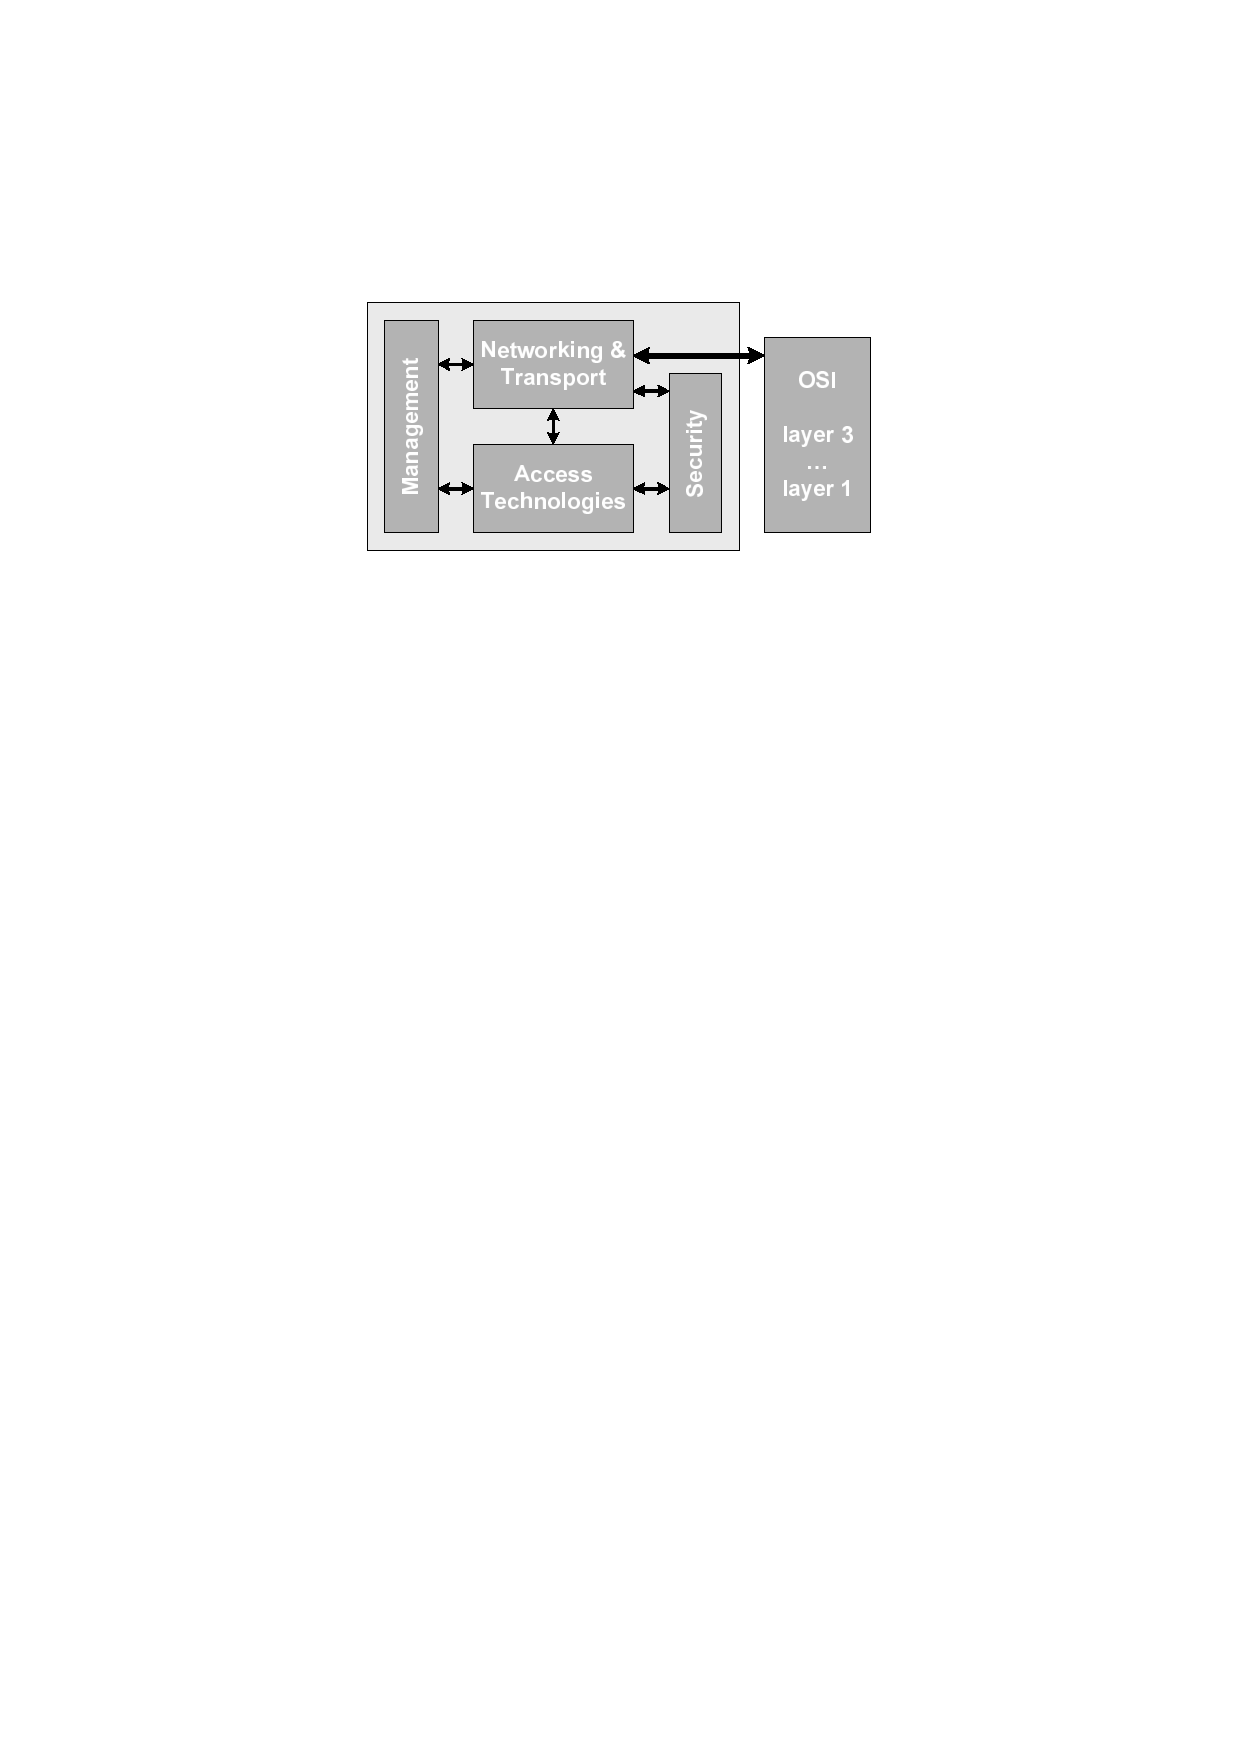
\includegraphics[width=0.99\textwidth]{content/images/01_funktionsweise/layer_borderRouter.pdf}
	\caption{Überblick über die Layer eines ITS Border Routers \cite{en302665}}
	\label{fig:funktionsweise_borderRouter}
\end{figure}



\section{Personal subsystem and station}
\ac{PSS} stellen die Funktionalitäten von \ac{ITS} in Geräten zur Verfügung, die in der Hand gehalten werden können. Der Standard nennt hierzu \ac{PDA} oder Mobiltelefone als Beispiel. Sie können als eigenständige Komponente dienen, oder als Teil einer anderen Komponente arbeiten.

\section{ITS Central Station}
Die \ac{ICS}, oder Central \ac{ITS} subsystem and station ist eine zentrale Komponente im \ac{ITS} System.

Die mindesten funktionalen Komponenten der \ac{ICS} sind:
\begin{itemize}
	\item \ac{ITS-S} Gateway \ref{funktionsweise_RoadsideITSGateway}
	\item \ac{ITS-S} Host \ref{funktionsweise_ITSHost}
	\item \ac{ITS-S} Border Router \ref{funktionsweise_ITSBorderRouter}
\end{itemize}

Die \ac{ICS} hat mehrere Aufgaben. Sie wird als Netzwerkknoten eingesetzt. Das bedeutet, dass sie die Daten, die von den \ac{IRS} empfangen wurden, zusammenführt. Sie kann aber auch die \ac{IRS} an das Core Network anbinden.

Eine weitere mögliche Funktion der \ac{ICS} ist die Funktion als Verkehrsleitzentrale. Dazu kann sie Applications hosten, die für die Steuerung des Verkehrsflusses verantwortlich sind. Vom baulichen her, kann sie auch die entsprechenden Arbeitsplätze für die Operatoren zur Verfügung stellen. 
	
	
\section{ITS Roadside Station}
Die Kommunikation ist nicht auf die Kommunikation von Fahrzeugen untereinander beschränkt. Eine Kommunikation zwischen Fahrzeugen und Verkehrsinfrastruktur ist ebenfalls möglich. Diese Kommunikation wird über \ac{IRS} oder \ac{RSU} abgewickelt. Da sie den Informationsfluss zwischen \ac{IVS} und \ac{ICS} ermöglicht, hat sie einen hohen Stellenwert im System. \ac{IRS} werden im Normalfall in bereits vorhandene Infrastruktur integriert. Hierfür bieten sich beispielsweise Ampeln oder sonstige Verkehrsleitsysteme an. 

Die \ac{IRS} beherrscht zwei grundlegend unterschiedliche Verbindungsprotokolle. Über das verbindungslose ITS-G5 kann die \ac{IRS} Verbindungen zu den \ac{IVS} aufbauen. Die Verbindung zu den \ac{ICS} erfolgt über TCP/IP. 

Eine \ac{IRS} besteht mindestens aus den folgenden funktionalen Komponenten:

\begin{itemize}
	\item  \ac{ITS-S} Gateway \ref{funktionsweise_RoadsideITSGateway}
	\item \ac{ITS-S} Host \ref{funktionsweise_ITSHost}
	\item \ac{ITS-S} Router \ref{funktionsweise_router}
	\item \ac{ITS-S} Border Router \ref{funktionsweise_ITSBorderRouter}
\end{itemize}

Neben der Funktion als reine Schnittstelle zwischen \ac{IRS} und \ac{IVS} kann die \ac{IRS} die empfangenen Daten aufbereiten, bzw. ein Function-Framework zur Verfügung stellen, auf dem Applikationen ausgeführt werden können. Die Funktionen des Function-Framework sind in der Beschreibung des Hosts \ref{funktionsweise_ITSHost} definiert.  

Beispiele für Applikationen der \ac{IRS} sind:
\begin{itemize}
	\item Store and Forward von Ereignisinformationen \ac{DENM}
	\item Weiterleitung von Ereignisinformationen an Versuchszentrale (Testzentrale)
	\item Aggregation von empfangenen Fahrzeugdaten zur Verbesserung der Wetter- und Verkehrslageerfassung
	\item Neue Anwendungen bzgl. der Interaktion zwischen Fahrzeug und LSA
	\item  Kreuzungsassistenz sowie Assistenz im Baustellenbereich
	\item Verteilung von Daten der ergänzenden Dienste aus der Versuchszentrale an die Fahrzeuge
	\item Versendung von Daten zur Kreuzungstopologie
\end{itemize}

Diese Beispiele sind aus einem Projektergebnis von \ac{SIMTD} entnommen (\cite{simtd-D12.1}). 



\section{ITS Vehicle Station}
Die \ac{IVS} ist eine mobile Komponente von \ac{ITS}. Sie hat als Mindestanforderung lediglich Schnittstellen in das \ac{ITS} Netzwerk und besteht mindestens aus folgenden funktionalen Komponenten:
\begin{itemize}
	\item  \ac{ITS-S} Gateway \ref{funktionsweise_RoadsideITSGateway}
	\item \ac{ITS-S} Host \ref{funktionsweise_ITSHost}
	\item \ac{ITS-S} Router \ref{funktionsweise_router} 
\end{itemize}

Eine \ac{IVS} wird in der Regel ein Fahrzeug sein. Die \ac{IVS} sind die Hauptteilnehmer der \ac{C2C}. Sie erfassen die Daten und übermitteln sie sich gegenseitig oder in das \ac{ITS} Netz. 
